\documentclass[12pt]{article}
\usepackage{times} 			% use Times New Roman font

\usepackage{parskip}

\usepackage[margin=1in]{geometry}   % sets 1 inch margins on all sides
\usepackage[hidelinks]{hyperref}               % for URL formatting
\usepackage[pdftex]{graphicx}       % So includegraphics will work
\setlength{\parskip}{1em}           % skip 1em between paragraphs
\usepackage{indentfirst}            % indent the first line of each paragraph
\usepackage{datetime}
\usepackage[small, bf]{caption}
\usepackage{listings}               % for code listings
\usepackage{xcolor}                 % for styling code
\usepackage{multirow}
\usepackage{subcaption}     % for subfigures

%\setlength\intextsep{1.69cm} 

%New colors defined below
\definecolor{backcolour}{RGB}{246, 246, 246}   % 0xF6, 0xF6, 0xF6
\definecolor{codegreen}{RGB}{16, 124, 2}       % 0x10, 0x7C, 0x02
\definecolor{codepurple}{RGB}{170, 0, 217}     % 0xAA, 0x00, 0xD9
\definecolor{codered}{RGB}{154, 0, 18}         % 0x9A, 0x00, 0x12

%Code listing style named "gcolabstyle" - matches Google Colab
\lstdefinestyle{gcolabstyle}{
  basicstyle=\ttfamily\small,
  backgroundcolor=\color{backcolour},   
  commentstyle=\itshape\color{codegreen},
  keywordstyle=\color{codepurple},
  stringstyle=\color{codered},
  numberstyle=\ttfamily\footnotesize\color{darkgray}, 
  breakatwhitespace=false,         
  breaklines=true,                 
  captionpos=b,                    
  keepspaces=true,                 
  numbers=left,                    
  numbersep=5pt,                  
  showspaces=false,                
  showstringspaces=false,
  showtabs=false,                  
  tabsize=2
}

\lstset{style=gcolabstyle}      %set gcolabstyle code listing

% to make long URIs break nicely
\makeatletter
\g@addto@macro{\UrlBreaks}{\UrlOrds}
\makeatother

% for fancy page headings
\usepackage{fancyhdr}
\setlength{\headheight}{13.6pt} % to remove fancyhdr warning
\pagestyle{fancy}
\fancyhf{}
\rhead{\small \thepage}
\chead{\small CS 532, Fall 2024} 
\lhead{\small HW2, Landers}  % EDIT THIS, REPLACE # with HW number

%-------------------------------------------------------------------------
\begin{document}

% EDIT THE ITEMS HERE
\begin{centering}
{\large\textbf{HW2 - Ranking Webpages}}\\ 
Ethan Landers\\
Due September 29th, 2024 by 11:59 PM\\
\end{centering}

%-------------------------------------------------------------------------

% The * after \section just says to not number the sections
\section*{Q1. Data Collection}

Q1 was divided into two parts: downloading and processing HTML content. I created two Python scripts to handle these tasks: download-html.py and process-html.py.

Download-html.py takes the URIs generated from Homework 1, generates an MD5 hash to use as the filename for each URI, downloads their corresponding HTML content, and then saves it to a file. A URI-to-hash mapping is also saved to a dictionary and written to uri\_mapping.txt. The bulk of the task was performed with the code below:

\begin{lstlisting}[language=Python, caption=download-html.py, label=lst:copy]
for uri in uris:
    hash_object = hashlib.md5(uri.encode())
    filename = f"{hash_object.hexdigest()}.html"

    try:
        response = requests.get(uri, timeout=5)
        with open(f"homework-2/raw_html/{filename}", 'w', encoding='utf-8') as file:
            file.write(response.text)

        uri_hash_map[filename] = uri

    except requests.exceptions.RequestException as e:
        print(f"Error fetching {uri}: \n{e}\n")

with open('homework-2/uri_mapping.txt', 'w', encoding='utf-8') as f:
    for filename, uri in uri_hash_map.items():
        f.write(f"{filename}: {uri}\n")
\end{lstlisting}

Next, I ran the process-html.py scrip to extract the main content from the raw HTML files using the extractor.get\_content() method from the BoilerPy3 library. If a file did not have meaningful content, it was skipped. The code below from process-html.py performs the bulk of the task:

\begin{lstlisting}[language=Python, caption=process-html.py, label=lst:copy]
for filename in os.listdir('homework-2/raw_html'):
    with open(f"homework-2/raw_html/{filename}", 'r', encoding='utf-8') as file:
        html_content = file.read()

    try:
        main_content = extractor.get_content(html_content)

        if main_content.strip():
            with open(f"homework-2/processed_html/{filename}", 'w', encoding='utf-8') as file:
                file.write(main_content)
            count = count + 1
        else:
            print(f"No useful content found in {filename}. Skipping.\n")

    except Exception as e:
        print(f"Error processing {filename}: {e}\n")
\end{lstlisting}

Q: How many of your 500 URIs produced useful text? If that number was less than 500, did that surprise you?

Out of 500 HTML files, 454 contained meaningful content. The remaining files were either empty or contained content that was not meaningful (e.g., navigation bars, footers, etc.) This result was unsurprising, as web pages often contain little relevant textual content for certain URIs.

\section*{Q2. Rank with TF-IDF}

I created a file called compute-tfidf.py, where I made two functions to calculate TF and IDF. 

The first function, compute\_tf(), computes TF by counting how many times a specific word appears in a document and dividing that number by the total number of words.

\begin{lstlisting}[language=Python]
def compute_tf(word, document):
    words = document.split()
    return words.count(word) / len(words) 
\end{lstlisting}

The second function, compute\_idf(), computes IDF by counting the number of times a specific query word appears in a document. Then, I divide the total number of processed HTML documents from question 1 by the number of documents with the query word. I then took log base 2 of the result, which provided the IDF. See the function below:

\begin{lstlisting}[language=Python]
def compute_idf(word, documents, total_docs_in_directory):
    num_docs_with_word = 0
    
    for doc in documents:
        if word in doc:
            num_docs_with_word += 1
    
    math.log((total_docs_in_directory) / (num_docs_with_word), 2)
\end{lstlisting}

The question required that I look for ten documents that contain a query word of my choice. I chose the query word "climate" because it is specific but not too general. I used grep in the command line to show me the first ten documents out of the HTML documents that had been processed before and contained the query "climate." The file names of the files that contained the query word were outputted. See below:

\begin{figure}[ht]
    \centering
    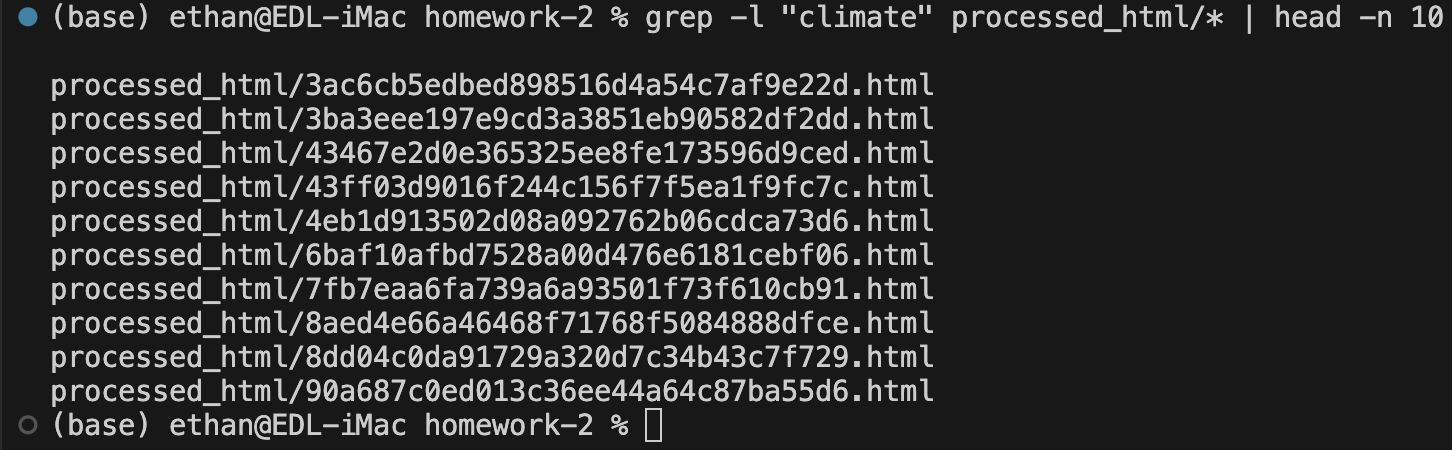
\includegraphics[width=1.0\textwidth]{grep.png} % Adjust width as needed
\end{figure}

I then manually added these files within a list within compute-tfidf.py to compute TF-IDF metrics.

\begin{lstlisting}[language=Python]
file_uris = [
    'homework-2/processed_html/3ac6cb5edbed898516d4a54c7af9e22d.html',
    'homework-2/processed_html/3ba3eee197e9cd3a3851eb90582df2dd.html',
    'homework-2/processed_html/43467e2d0e365325ee8fe173596d9ced.html',
    'homework-2/processed_html/43ff03d9016f244c156f7f5ea1f9fc7c.html',
    'homework-2/processed_html/4eb1d913502d08a092762b06cdca73d6.html',
    'homework-2/processed_html/6baf10afbd7528a00d476e6181cebf06.html',
    'homework-2/processed_html/7fb7eaa6fa739a6a93501f73f610cb91.html',
    'homework-2/processed_html/8aed4e66a46468f71768f5084888dfce.html',
    'homework-2/processed_html/8dd04c0da91729a320d7c34b43c7f729.html',
    'homework-2/processed_html/90a687c0ed013c36ee44a64c87ba55d6.html'
]
\end{lstlisting}

From there, I computed TF, IDF, and TF-IDF, then appended those results to a list to hold those results for each URI. 

\begin{lstlisting}[language=Python]
directory_path = 'homework-2/processed_html'

total_docs_in_directory = len([doc for doc in os.listdir(directory_path)])

documents = {}

for uri in file_uris:
    with open(uri, 'r', encoding='utf-8') as file:
        documents[uri] = file.read()

tf_idf_results = []

for uri, document in documents.items():
    tf = compute_tf(query_term, document)
    idf = compute_idf(query_term, documents.values(), total_docs_in_directory)
    tf_idf = tf * idf
    tf_idf_results.append((tf_idf, tf, idf, uri))
\end{lstlisting}

I then wrote the results to the terminal sorted by TF-IDF, and below in the table are those same results:

\begin{table}[h]
\centering
\caption{10 Hits for the term "climate", ranked by TF-IDF}
\label{tbl:simple}
\begin{tabular}{|l|l|l|l|}
\hline
\textbf{TF-IDF} & \textbf{TF} & \textbf{IDF} & \textbf{URI} \\ \hline \hline
0.1102 & 0.0200 & 5.5110 & https://www.odu.edu/ \\ \hline
0.0380 & 0.0069 & 5.5110 & https://news-un-org.translate.goog/en/ \\ \hline
0.0357 & 0.0065 & 5.5110 & https://news-un-org.translate.goog/en/ \\ \hline
0.0306 & 0.0056 & 5.5110 & https://news-un-org.translate.goog/en/ \\ \hline
0.0277 & 0.0050 & 5.5110 & https://www.odu.edu/ \\ \hline
0.0239 & 0.0043 & 5.5110 & https://news-un-org.translate.goog/en/ \\ \hline
0.0202 & 0.0037 & 5.5110 & https://www-leibniz--gemeinschaft-de.translate.goog/en \\ \hline
0.0120 & 0.0022 & 5.5110 & https://news-un-org.translate.goog/en/ \\ \hline
0.0120 & 0.0022 & 5.5110 & https://www-leibniz--gemeinschaft-de.translate.goog/en \\ \hline
0.0042 & 0.0008 & 5.5110 & https://www-leibniz--gemeinschaft-de.translate.goog/en \\ \hline
\end{tabular}
\end{table}

Please note that I shortened the URIs to contain only the most essential parts for report conciseness purposes.

Looking at these results, one of the odu.edu links using the query term "climate" is more important than the other URIs, with the highest TF-IDF of 0.1102. It also has the highest TF, meaning the term "climate" appears the most in that URI compared to all the others. The other URIs have the query term "climate," but its frequency may be less.

\section*{Q3. Rank with PageRank}

For the ten URIs that contained the query term "climate," I entered them into the page ranking tool \url{https://searchenginereports.net/google-pagerank-checker} to see what their page ranking is.

I then created a script called pagerank.py, in which I first manually created a dictionary containing the PageRank values of each of the ten URIs.

\begin{lstlisting}[language=Python]
pagerank_values = {
    "https://www.odu.edu/oir": 7,
    "https://news-un-org.translate.goog/en/?_x_tr_sl=en&_x_tr_tl=ru": 6,
    "https://news-un-org.translate.goog/en/focus/mali?_x_tr_sl=en&_x_tr_tl=ru": 6,
    "https://news-un-org.translate.goog/en/content/un-news-go?_x_tr_sl=en&_x_tr_tl=ru": 6,
    "https://www.odu.edu/research-0": 7,
    "https://news-un-org.translate.goog/en/un-podcasts?_x_tr_sl=en&_x_tr_tl=ru": 6,
    "https://www-leibniz--gemeinschaft-de.translate.goog/en/about-us/whats-new/news/forschungsnachrichten-single/newsdetails/solidaritaet-mit-der-ukraine?_x_tr_sl=en&_x_tr_tl=uk": 0,
    "https://news-un-org.translate.goog/en/news/topic/climate-change?_x_tr_sl=en&_x_tr_tl=ru": 6,
    "https://www-leibniz--gemeinschaft-de.translate.goog/en/about-us/whats-new/news/forschungsnachrichten-single/newsdetails/solidaritaet-mit-der-ukraine?_x_tr_sl=en&_x_tr_tl=ru": 0,
    "https://www-leibniz--gemeinschaft-de.translate.goog/en/about-us/whats-new/news?_x_tr_sl=en&_x_tr_tl=uk": 0,
}
\end{lstlisting}

I then took the minimum and maximum of these PageRank values to normalize them to a scale from 0 to 1. I then wrote the URIs and their normalized PageRank values to the terminal, and the table below shows the PageRank values:

\begin{table}[h]
\centering
\caption{10 hits for the term "climate", ranked by PageRank of domain.}
\label{tbl:simple}
\begin{tabular}{|l|l|}
\hline
\textbf{PageRank} & \textbf{URI} \\ \hline \hline
1.0 & https://www.odu.edu/ \\ \hline
0.9 & https://news-un-org.translate.goog/en/ \\ \hline
0.9 & https://news-un-org.translate.goog/en/ \\ \hline
0.9 & https://news-un-org.translate.goog/en/ \\ \hline
1.0 & https://www.odu.edu/ \\ \hline
0.9 & https://news-un-org.translate.goog/en/ \\ \hline
0.0 & https://www-leibniz--gemeinschaft-de.translate.goog/en/ \\ \hline
0.9 & https://news-un-org.translate.goog/en/ \\ \hline
0.0 & https://www-leibniz--gemeinschaft-de.translate.goog/en/ \\ \hline
0.0 & https://www-leibniz--gemeinschaft-de.translate.goog/en/ \\ \hline

\end{tabular}
\end{table}

Q: Briefly compare and contrast the rankings produced in Q2 and Q3.

TF-IDF measures the importance of the query term "climate" in each document relevant to the corpus of documents. The URI www.odu.edu had the highest TF-IDF of 0.1102, signifying the term is highly relevant.

PageRank measures how many other websites link to a URI and isn't concerned with a query term like "climate." www.odu.edu has a high PageRank value, suggesting it is a trusted and credible website. Some websites, like https://www-leibniz–gemeinschaft-de.translate.goog/en/, had a PageRank of zero after normalizing, signifying that it is much less linked to.

So, URIs with a high TF-IDF score and PageRank value, like www.odu.edu, are highly relevant because they are content-relevant and come from websites often linked to. A high PageRank value but a lower TF-IDF score signifies that a URI is credible but might not be relevant. When both TF-IDF and PageRank values are low, they are neither relevant nor credible.

\section*{References}

\begin{itemize}
    \item{BoilerPy3, \url{https://pypi.org/project/boilerpy3/}}
    \item{Data Normalization Techniques, \url{https://analystanswers.com/data-normalization-techniques-easy-to-advanced-the-best/}}
    \item {Page Ranking Tool, \url{https://searchenginereports.net/google-pagerank-checker}}
    \item{Python Hashing, \url{https://www.geeksforgeeks.org/md5-hash-python/}}
    \item{Python shutil.rmtree() method, \url{https://www.geeksforgeeks.org/delete-an-entire-directory-tree-using-python-shutil-rmtree-method/}}
\end{itemize}

\end{document}

